\section{Banded trigonometric function}
\label{sec:banded_trigonometric_results}

The banded trigonometric function is defined as follows.
\begin{equation}
f(x) = \sum_{i=1}^n i[(1-\cos x_i) + \sin x_{i-1} - \sin x_{i+1}]
\end{equation}
Figure \ref{fig:banded_trigonometric_surf} shows the surface plot of the 2-dimensional banded trigonometric function.
It has a highly oscillatory landscape with multiple peaks and valleys due to its sinusoidal terms.
This results in a mix of locally smooth and rapidly changing regions, making optimization sensitive to initialization and prone to multiple local minima.
\begin{figure}
    \centering
    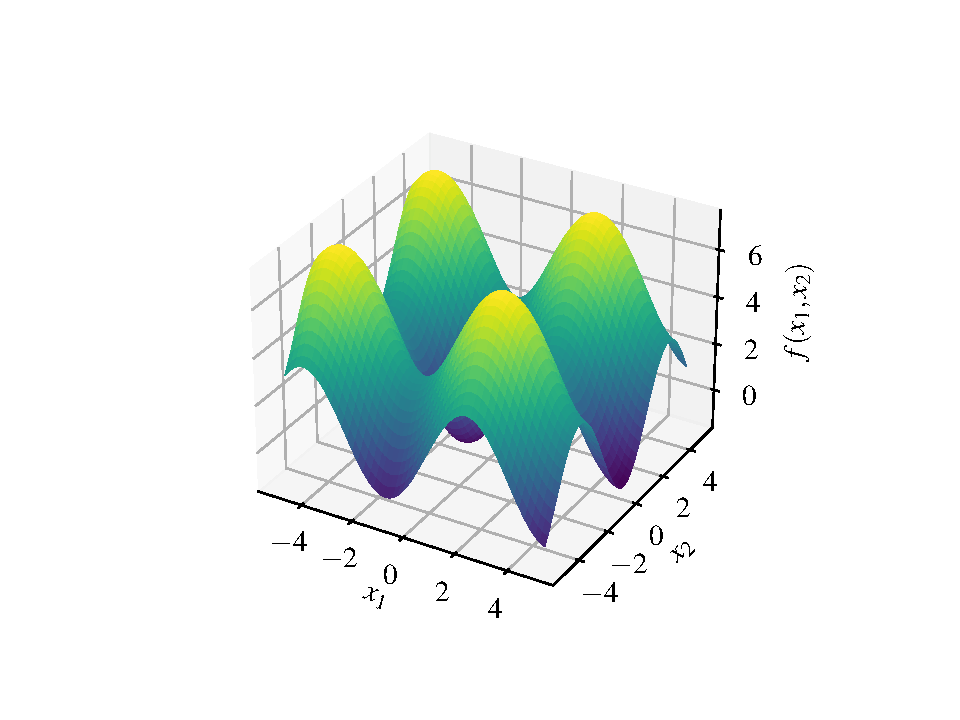
\includegraphics[width=0.5\textwidth]{figures/banded_trigonometric_surf.pdf}
    \caption{Surface plot of the 2-dimensional banded trigonometric function}
    \label{fig:banded_trigonometric_surf}
\end{figure}
The optimization runs for the banded trigonometric function were conducted using a high value for the Armijo condition parameter $c_1 = 10^{-2}$ while the other parameters were kept the same as in the previous experiments.
This was necessary since when running the modified Newton method, the too small required decrease led to stagnation.

\subsection{Exact gradient and Hessian}

The gradient of the banded trigonometric function is given by the following expression.
\begin{equation}
\frac{\partial F}{\partial x_k} = \left \{ \begin{array}{ll}
k\sin x_k + 2\cos x_k, & 1 \leq k < n \\
n\sin x_n - (n-1)\cos x_n, & k = n
\end{array} \right .
\end{equation}
The Hessian of the banded trigonometric function is given by the following expression.
\begin{equation}
\frac{\partial^2 F}{\partial x_k \partial x_j} = \left \{ \begin{array}{ll}
    k\cos x_k - 2\sin(x_k), & 1\leq k = j < n \\
    n\cos x_n + (n-1)\sin x_n, & k = j = n \\
    0, & \text{otherwise}
\end{array} \right .
\end{equation}
Notice that the Hessian is a diagonal matrix, which makes the optimization problem easier to solve.
However, the Hessian of the matrix has very distant eigenvalues due to the fact that the $i$-th diagonal entry is multiplied by $i$: the problem may become increasingly ill-conditioned as the dimension $n$ increases.
Due to this fact, we only perform optimization with preconditioning.

Table \ref{tab:Modified_Newton_Banded_Trigonometric_exact} shows the results for the \textit{Modified Newton method} applied to the banded trigonometric function with exact gradient and Hessian.
Modified newton method converges for all points when $n=10^3$ or $n=10^4$, while attempts with $n=10^5$ yield only one success corresponding to the suggested starting point.
When problem dimension is $n=10^5$, attempts with randomly initialized points do not converge within $k_{\textit{max}} = 10^3$ iterations.
This may be due to the fact that being the problem badly scaled, in case of a non positive-definite Hessian matrix, the modification of the Hessian matrix may happen with a $\tau$ that is too large.
Figure \ref{fig:correction_comparison} compares the empirical cumulative distribution function of $\tau_k$ for the banded trigonometric problem and the extended Rosenbrock function with exact gradient and Hessian.
One can notice that while for the extended Rosenbrock function the maximum value of the correction does not depend on the dimension, for the banded trigonometric problem the maximum value of the correction increases with the dimension.
Moreover, as suggested by the factor $i$ that multiplies the $i$-th diagonal entry of the Hessian, the maximum correction needed for the dimension $10^n$ is close to $10^n$.
While a correction of this magnitude is acceptable for $n=10^3$ or $n=10^4$, it is not for larger values of $n$, leading to a Hessian matrix that is too different from the original one and resulting in a poor descent direction.
All failures happen because convergence has not been reached within $k_{\textit{max}} = 10^3$ iterations.

\begin{table}
\centering
\caption{Results for Modified Newton method applied to Banded Trigonometric with exact gradient and hessian, metrics are average metrics for succesful attempts. Results are given only with preconditioning adopted.}
\label{tab:Modified_Newton_Banded_Trigonometric_exact}
\begin{tabular}{r|cccc}
\toprule
dimension & iterations & convergence rate & time & success rate \\
\midrule
3 & 27.273 & 2.593 & 0.025 & 1.00 \\
4 & 51.545 & 2.749 & 0.150 & 1.00 \\
5 & 7.000 & 2.946 & 0.092 & 0.09 \\
\bottomrule
\end{tabular}
\end{table}

\begin{figure}
    \centering
    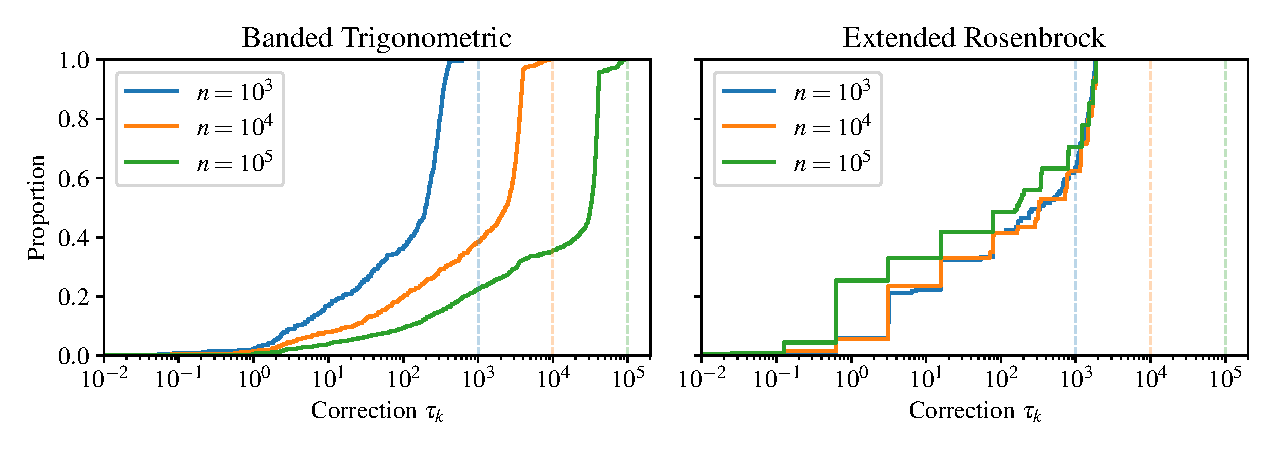
\includegraphics[width=0.9\textwidth]{figures/correction_comparison.pdf}
    \caption{Emprirical cumulative distribution function of $\tau_k$ in banded trigonometric problem and extended Rosenbrock function with exact gradient and Hessian, considering all times a correction is needed across all runs. Dashed lines mark the values $10^3$, $10^4$ and $10^5$.}
    \label{fig:correction_comparison}
\end{figure}

Table \ref{tab:Truncated_Newton_Banded_Trigonometric_exact} shows the results for the \textit{Truncated Newton method} applied to the banded trigonometric function with exact gradient and Hessian.
All attempts are succesful, and the method converges in a small number of iterations with a large experimental rate of convergence.
So, when preconditioning is adopted, the Truncated Newton method is able to solve the problem efficiently unlike Modified Newton method.
Probably adopting another matrix correction strategy that impacts less on the whole matrix, such as the one based on \textit{Modified Cholesky factorization} proposed in \cite{nocedal-optimization}, could lead to better results.

\begin{table}
\centering
\caption{Results for Truncated Newton method applied to Banded Trigonometric with exact gradient and hessian, metrics are average metrics for succesful attempts. Results are given only with preconditioning adopted.}
\label{tab:Truncated_Newton_Banded_Trigonometric_exact}
\begin{tabular}{r|cc|cc}
\toprule
dimension & iterations & convergence rate & time & success rate \\
\midrule
3 & 14.091 & 2.811 & 0.009 & 1.00 \\
4 & 20.455 & 2.743 & 0.028 & 1.00 \\
5 & 25.000 & 2.776 & 0.301 & 1.00 \\
\bottomrule
\end{tabular}
\end{table}

\subsection{Finite differences gradient and Hessian}

When applying \ref{eq:findiff_gradient}, one can notice that the terms $F(x + he_k)$ and $F(x - he_k)$ only differ by summands with indices $i = k$ and $i = k \pm 1$.
Then to make function evaluations less expensive, we can define the following function $F_{\textit{fd},\,k}$, that can be plugged in \ref{eq:findiff_gradient} in place of $F$ yielding the same result.
\[
F_{\textit{fd},\,k} = \sum_{i=k-1}^{k+1} i[(1-\cos x_i) + \sin x_{i-1} - \sin x_{i+1}]
\]
Some of the terms in $F_{fd,\,k}$ are constant and do not depend on $x_k$, so they will eventually subtract and we can further simplify the expression.
\[
F_{\textit{fd},\,k} = \left \{ \begin{array}{ll}
    -k\cos x_k + 2\sin x_k, & 1 \leq k < n \\
    n\cos x_n - (n-1)\sin x_n, & k = n
\end{array} \right .
\]
The same procedure can be applied to the Hessian, considering that terms in \ref{eq:findiff_hessian} only differ by summands with indices $i = k$ and $i = k \pm 1$.
When plugging the function $F_{\textit{fd},\,k}$ into \ref{eq:findiff_gradient} and \ref{eq:findiff_hessian} it's convenient to expand them so that the computation of the gradient and Hessian is not subject to numerical cancellation.
After expanding the functions, the gradient and Hessian can be approximated as follows.
\begin{align*}
    \frac{\partial F}{\partial x_k} &\approx \left \{ \begin{array}{ll}
        \frac{2k\sin x_k \sin h + 4\cos x_k \sin h}{2h}, & 1 \leq k < n \\
        \frac{2n\sin x_n \sin h - 2(n-1)\cos x_k \sin h}{2h}, & k = n
    \end{array} \right . \\
    \frac{\partial^2 F}{\partial x_k^2} &\approx \left \{ \begin{array}{ll}
        (k\cos x_k - 2\sin x_k) - h(k\sin x_k + 2\cos x_k), 
        & 1 \leq k < n \\
        (n\cos x_n - (n-1)\sin x_n) - h(n\sin x_n - (n-1)\cos x_n),
        & k = n
    \end{array} \right .
\end{align*}
The approximation for the gradient is obtained applying the trigonometric identities for the sum of angles.
The approximation for the Hessian is obtained by applying the aforementioned trigonometric identities in order to isolate the following terms.
\[
\cos(2h) - 2\cos h \approx -1 - h^2 + \mathcal{O}(h^4),
\qquad
\sin(2h) - 2\sin h \approx -h^3 + \mathcal{O}(h^5)
\]
To avoid numerical cancellation, it is necessary to substitute them with their Taylor expansions.

Tables \ref{tab:Modified_Newton_Banded_Trigonometric_fd_abs} and \ref{tab:Modified_Newton_Banded_Trigonometric_fd_rel} show the results for the \textit{Modified Newton method} applied to the banded trigonometric function with absolute and specific finite differences, respectively.
In terms of success rate, results are comparable to the ones obtained with exact gradient and Hessian.
However, when specific finite differences are adopted, approximation with $h=10^{-2}$, $h=10^{-4}$ and $h=10^{-6}$ give poor results, with success rate for $h=10^{-2}$ being 0\% for all dimension.
On the other hand, when increments are constant, we get at least 9\% success rate for all dimensions, all increments and 100\% success rate when $n=10^{4}$ or $n=10^{5}$.
When absolute increment is adopted, all failures happen due to the fact that convergence has not been reached within $k_{\textit{max}} = 10^3$ iterations.
When specific increment is adopted, most failures happen because the method does not converge within $k_{\textit{max}} = 10^3$ iterations, but in 1 case over 18 failures for $n=10^{3}$, 4 cases over 24 failures for $n=10^4$ and in 3 cases over 61 failures for $n=10^5$, failure happens because Armijo condition can't be satisfied.

\begin{table}
\centering
\caption{Results for Modified Newton method applied to Banded Trigonometric with finite differences and constant increment, metrics are average metrics for succesful attempts. Results are given only with preconditioning adopted.}
\label{tab:Modified_Newton_Banded_Trigonometric_fd_abs}
\begin{tabular}{rr|cccc}
\toprule
    &  & iterations & convergence rate & time & success rate \\
dimension & h &  &  &  &  \\
\midrule
\multirow[t]{6}{*}{3} & 1e-02 & 27.364 & 2.676 & 0.018 & 1.00 \\
    & 1e-04 & 27.545 & 2.743 & 0.014 & 1.00 \\
    & 1e-06 & 25.909 & 2.807 & 0.013 & 1.00 \\
    & 1e-08 & 27.818 & 2.467 & 0.015 & 1.00 \\
    & 1e-10 & 27.182 & 2.770 & 0.014 & 1.00 \\
    & 1e-12 & 27.182 & 2.817 & 0.015 & 1.00 \\
\cline{1-6}
\multirow[t]{6}{*}{4} & 1e-02 & 60.818 & 2.661 & 0.179 & 1.00 \\
    & 1e-04 & 50.091 & 2.626 & 0.149 & 1.00 \\
    & 1e-06 & 54.364 & 2.831 & 0.161 & 1.00 \\
    & 1e-08 & 49.091 & 2.770 & 0.152 & 1.00 \\
    & 1e-10 & 51.364 & 2.767 & 0.149 & 1.00 \\
    & 1e-12 & 51.909 & 2.516 & 0.157 & 1.00 \\
\cline{1-6}
\multirow[t]{6}{*}{5} & 1e-02 & 9.000 & 2.705 & 0.129 & 0.09 \\
    & 1e-04 & 8.000 & 2.828 & 0.113 & 0.09 \\
    & 1e-06 & 6.000 & 2.856 & 0.085 & 0.09 \\
    & 1e-08 & 6.000 & 2.749 & 0.088 & 0.09 \\
    & 1e-10 & 7.000 & 2.948 & 0.098 & 0.09 \\
    & 1e-12 & 7.000 & 2.946 & 0.099 & 0.09 \\
\cline{1-6}
\bottomrule
\end{tabular}
\end{table}

\begin{table}
\centering
\caption{Results for Modified Newton method applied to Banded Trigonometric with finite differences and specific increment, metrics are average metrics for succesful attempts. Results are given only with preconditioning adopted.}
\label{tab:Modified_Newton_Banded_Trigonometric_fd_rel}
\begin{tabular}{rr|cccc}
\toprule
    &  & iterations & convergence rate & time & success rate \\
dimension & h &  &  &  &  \\
\midrule
\multirow[t]{5}{*}{3} & 1e-04 & 162.000 & 0.984 & 0.050 & 0.36 \\
    & 1e-06 & 26.818 & 2.389 & 0.014 & 1.00 \\
    & 1e-08 & 27.000 & 2.610 & 0.015 & 1.00 \\
    & 1e-10 & 27.091 & 2.597 & 0.014 & 1.00 \\
    & 1e-12 & 27.273 & 2.820 & 0.015 & 1.00 \\
\cline{1-6}
\multirow[t]{5}{*}{4} & 1e-04 & 9.000 & 0.973 & 0.018 & 0.09 \\
    & 1e-06 & 55.875 & inf & 0.161 & 0.73 \\
    & 1e-08 & 50.636 & 2.791 & 0.152 & 1.00 \\
    & 1e-10 & 51.091 & 2.617 & 0.152 & 1.00 \\
    & 1e-12 & 51.273 & 2.684 & 0.152 & 1.00 \\
\cline{1-6}
\multirow[t]{5}{*}{5} & 1e-04 & 9.000 & 1.074 & 0.128 & 0.09 \\
    & 1e-06 & 6.000 & 2.894 & 0.083 & 0.09 \\
    & 1e-08 & 6.000 & 2.749 & 0.085 & 0.09 \\
    & 1e-10 & 7.000 & 2.948 & 0.095 & 0.09 \\
    & 1e-12 & 7.000 & 2.946 & 0.098 & 0.09 \\
\cline{1-6}
\bottomrule
\end{tabular}
\end{table}

Tables \ref{tab:Truncated_Newton_Banded_Trigonometric_fd_abs} and \ref{tab:Truncated_Newton_Banded_Trigonometric_fd_rel} show the results for the \textit{Truncated Newton method} applied to the banded trigonometric function with absolute and specific finite differences, respectively.
All attempts are succesful, and the method converges in a small number of iterations with a large experimental rate of convergence.
The results are similar to the ones obtained with exact gradient and Hessian, confirming that the Truncated Newton method is a suitable algorithm to tackle the banded trigonometric problem optimization.

\begin{table}
\centering
\caption{Results for Truncated Newton method applied to Banded Trigonometric with finite differences and constant increment, metrics are average metrics for succesful attempts. Results are given only with preconditioning adopted.}
\label{tab:Truncated_Newton_Banded_Trigonometric_fd_abs}
\begin{tabular}{rr|cccc}
\toprule
    &  & iterations & convergence rate & time & success rate \\
dimension & h &  &  &  &  \\
\midrule
\multirow[t]{6}{*}{3} & 1e-02 & 14.909 & 2.723 & 0.007 & 1.00 \\
    & 1e-04 & 14.091 & 2.615 & 0.006 & 1.00 \\
    & 1e-06 & 14.091 & 2.531 & 0.005 & 1.00 \\
    & 1e-08 & 14.091 & 2.770 & 0.006 & 1.00 \\
    & 1e-10 & 14.000 & 2.794 & 0.005 & 1.00 \\
    & 1e-12 & 14.000 & 2.779 & 0.006 & 1.00 \\
\cline{1-6}
\multirow[t]{6}{*}{4} & 1e-02 & 19.091 & 2.595 & 0.028 & 1.00 \\
    & 1e-04 & 19.364 & 2.587 & 0.028 & 1.00 \\
    & 1e-06 & 20.091 & 2.646 & 0.028 & 1.00 \\
    & 1e-08 & 20.636 & 2.741 & 0.030 & 1.00 \\
    & 1e-10 & 20.364 & 2.798 & 0.028 & 1.00 \\
    & 1e-12 & 20.455 & 2.758 & 0.028 & 1.00 \\
\cline{1-6}
\multirow[t]{6}{*}{5} & 1e-02 & 23.000 & 2.471 & 0.301 & 0.91 \\
    & 1e-04 & 25.909 & 2.648 & 0.315 & 1.00 \\
    & 1e-06 & 25.727 & 2.612 & 0.327 & 1.00 \\
    & 1e-08 & 25.636 & 2.762 & 0.313 & 1.00 \\
    & 1e-10 & 25.364 & 2.754 & 0.312 & 1.00 \\
    & 1e-12 & 25.273 & 2.699 & 0.311 & 1.00 \\
\cline{1-6}
\bottomrule
\end{tabular}
\end{table}

\begin{table}
\centering
\caption{Results for Truncated Newton method applied to Banded Trigonometric with finite differences and specific increment, metrics are average metrics for succesful attempts. Results are given only with preconditioning adopted.}
\label{tab:Truncated_Newton_Banded_Trigonometric_fd_rel}
\begin{tabular}{rr|cccc}
\toprule
    &  & iterations & convergence rate & time & success rate \\
dimension & h &  &  &  &  \\
\midrule
\multirow[t]{6}{*}{3} & 1e-02 & 15.000 & 2.251 & 0.005 & 1.00 \\
    & 1e-04 & 15.091 & 2.860 & 0.006 & 1.00 \\
    & 1e-06 & 13.818 & 2.534 & 0.006 & 1.00 \\
    & 1e-08 & 13.818 & 2.609 & 0.006 & 1.00 \\
    & 1e-10 & 14.000 & 2.795 & 0.006 & 1.00 \\
    & 1e-12 & 14.000 & 2.803 & 0.006 & 1.00 \\
\cline{1-6}
\multirow[t]{6}{*}{4} & 1e-02 & 19.909 & 2.118 & 0.027 & 1.00 \\
    & 1e-04 & 19.182 & 2.666 & 0.026 & 1.00 \\
    & 1e-06 & 20.455 & 2.851 & 0.028 & 1.00 \\
    & 1e-08 & 20.182 & 2.650 & 0.028 & 1.00 \\
    & 1e-10 & 19.818 & 2.811 & 0.027 & 1.00 \\
    & 1e-12 & 19.909 & 2.699 & 0.027 & 1.00 \\
\cline{1-6}
\multirow[t]{6}{*}{5} & 1e-02 & 24.273 & 2.351 & 0.313 & 1.00 \\
    & 1e-04 & 25.364 & 2.715 & 0.295 & 1.00 \\
    & 1e-06 & 26.455 & 2.748 & 0.315 & 1.00 \\
    & 1e-08 & 25.364 & 2.717 & 0.321 & 1.00 \\
    & 1e-10 & 25.455 & 2.713 & 0.315 & 1.00 \\
    & 1e-12 & 25.091 & 2.549 & 0.308 & 1.00 \\
\cline{1-6}
\bottomrule
\end{tabular}
\end{table}